\section{Synthesizers}

\subsection{Roland D-50}
The Roland D-50 is a polyphonic 61-key synthesizer produced by Roland in 1987. It features Linear Arithmetic synthesis, onboard effects, a joystick, and analog synthesis-styled layout. Linear Arithmetic synthesis combines sample playback with digital synthesis. Roland used samples to simulate the most realistic attack and then the D-50 uses the synthesizer section to sustain the sound. This method saved on the expense of RAM and gave the synthesized sound a texture that made it popular with choir, wind, and string patches. Notable users are: 808 State, Alphaville, Aphex Twin, Enya, Duran Duran, George Michael, Michael Jackson, Phil Collins, Prince, and Rush. \\
\linebreak
\href{https://github.com/dkadyrov/MIDILab/blob/master/Manuals/Roland_D50.pdf}{Roland D-50 Manual (PDF)}

\begin{figure}[h]
\centering
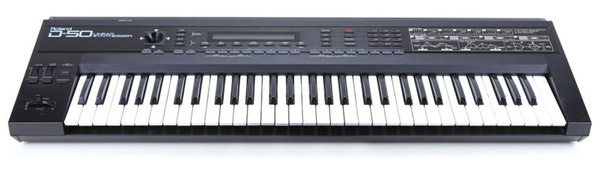
\includegraphics[width=.85\textwidth]{Images/roland_d50.jpg}
\caption{Roland D-50}
\label{fig:fullfig}
\end{figure}

\textbf{Quick Patching}
\begin{enumerate}
	\item Select the bank number with the numbers on the lower left side
	\item Select the patch number within the ban with the numbers on the lower right side
	\item Press [PATCH EDIT] and select the parameters to change in the menu
	\item The Modulation Bender and [PORTAMENTO] on the left side allow for live changes
\end{enumerate}

\newpage
\subsection{Korg Triton Extreme}
The Korg Triton made its debut in 2004. It is a workstation and sampler (16 MB sample RAM, 2 minutes and 54 seconds in mono at 48 kHz), has a programmable arpeggiator, ribbon controller, 2 USB ports, and "Valve Force" which can convert the signal into analog form. Notable users are: David Bowie, Coldplay, Lady Gaga, Ronald Jenkees, Linkin Park, Moby, Paul Oakenfold, Scooter, Mike Shinoda, Serj Tankian, and Timbaland. \\
\linebreak
\href{https://github.com/dkadyrov/MIDILab/blob/master/Manuals/Korg_Triton_Extreme.pdf}{Korg Triton Extreme Manual (PDF)}

\begin{figure*}[h]
\centering
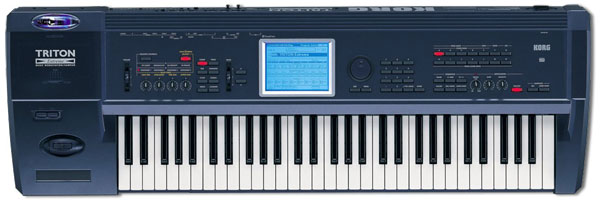
\includegraphics[width=.85\textwidth]{Images/tritonextreme.jpg}
\caption{Korg Triton Extreme}
\label{fig:fullfig}
\end{figure*}

\textbf{Edit Suggestions}
\begin{enumerate}
	\item Press [PROG] (Program) Mode
	\item Press Bank \& Program keys, turn dial, use touchscreen or use up and down keys to select patches.
	\item Press [MENU]
	\item Press [REAL TIME CONTROLS]
\end{enumerate}

\textbf{Add Effects}
\begin{enumerate}
	\item Press [MENU] key, Page Jump Menu, press P8 (or hold MENU key down)
	\item Press routing tab in window, choose IFX
	\item Press Insert FX tab at the bottom of the window and choose a tab at the bottom of the window
	\item Choose desired effect (change to ON by pressing OFF button)
	\item Check CHAIN box to add another effect; press OFF button of that effect to change to ON
\end{enumerate}

\newpage

\newpage

\subsection{E-mu Proteus 2000}

	The E-mu Proteus 2000 was released in 1999. Contains thousands of waves utilizing 32 MB of ROM. Features 128 voice polyphony and 32-part multi-timbrality. E-mu Systems became a popular company with their Emulator sampler and continued to pioneer sample-based synthesis with the Proteus range. The sampler does not allow users to record sounds, but offers a range of factory sounds that then can be layered, filtered, modulated by LFO's, and shaped by envelopes. \\
\linebreak
\href{https://github.com/dkadyrov/MIDILab/blob/master/Manuals/EMU_Proteus2000.pdf}{E-mu Proteus 2000 Manual (PDF)}


\begin{figure*}[h]
\centering
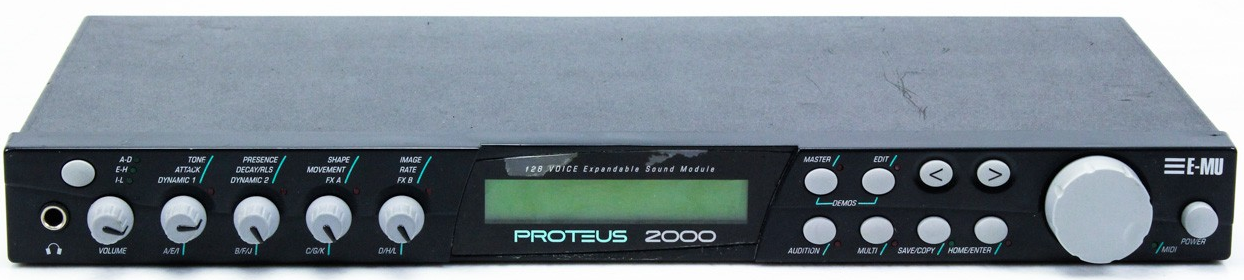
\includegraphics[width=.85\textwidth]{Images/e-mu-proteus-2000}
\caption{E-mu Proteus 2000}
\label{fig:fullfig}
\end{figure*}

\textbf{Quick Patching}
\begin{enumerate}
	\item Turn the large knob (data entry knob) to switch through patches
	\item Change parameters with the 5 smaller knobs (realtime control knobs) on the left side. The button to the left of the realtime control knobs changes the function of the row of knobs (written list above knobs).
	\item For more complex control, press the [EDIT] button and use the data entry knob to select the parameters you want to change. Press the in the data entry knob as an enter function and then change the data values by turning the knob.
\end{enumerate}
